\chapter{Casos de Estudio}
\label{cap:casos}

Es interesante realizar una evaluación simple, al menos de una forma empírica, de la utilidad de la aplicación Web. 

La aplicación complementa el desarrollo de la metodología de detección propuesta e intenta presentar la información junto a su contexto, es decir, evitando reducir la detección a una alerta de sismo, si no más bien, presentar los datos recolectados de la forma más completa e intuitiva posible para que los usuarios puedan interpretar su significado y determinar su utilidad.

En este capítulo se presentan algunos casos de estudio que muestran cómo se visualizó la información en la aplicación Web durante algunos sismos. 
Los casos presentados corresponden a un sismo en Chile, algunos casos de sismos en otros países y además se incluye un caso correspondiente a un caso falso positivo.

Finalmente se incluye una breve conclusión respecto a la utilidad de la aplicación Web.

	\section{Caso I: Sismo al sur de Chile}	
	
	\begin{figure}[!h]
	  \centering
	  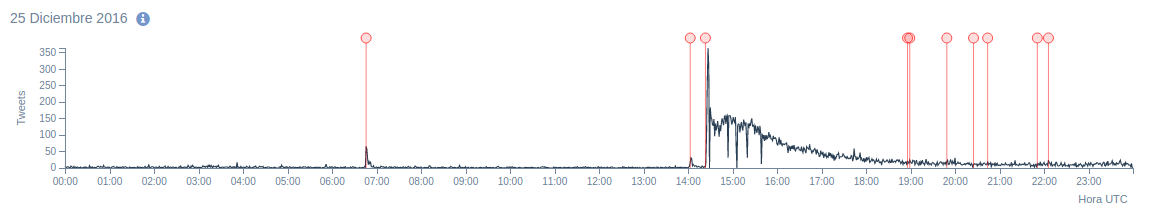
\includegraphics[width=\textwidth]{imagenes/img-25Dic-freq.png}
	  \caption{Frecuencia de mensajes relacionados con sismos durante el 25 de Diciembre del 2016.}
		\label{fig:timeline-25Dic}
	\end{figure}
	
	
	A las 14:24:30 hrs. del 25 de Diciembre del 2016 el sistema de detección basado en redes sociales detectó  un evento sísmico. La figura \ref{fig:timeline-25Dic} muestra la frecuencia de mensajes y el tercer marcador rojo, coincide con la detección antes mencionada. Los primeros \textit{tweets} publicados que mencionaban el suceso daban cuenta de que el sismo se percibía fuerte en Puerto Montt. A continuación se mencionan los 5 primeros mensajes publicados en la red social relacionados a este evento. 


\textit{``Temblor fuerte en Puerto mont'' $@$ginniasa, 14:23:27, 25/12/16}

\textit{``Está temblando heavy'' $@$loremba, 14:23:33 25/12/16}

\textit{``Dónde me duerma no me despierta ni un terremoto'' $@$SolRostan, 14:23:34 25/12/16}

\textit{``Temblando'' $@$fredyvargasr, 14:23:48 25/12/16}

\textit{``Temblor en \#puertomontt'' $@$correos73, 14:23:50 25/12/16}

	\begin{figure}[!ht]
	  \centering
	  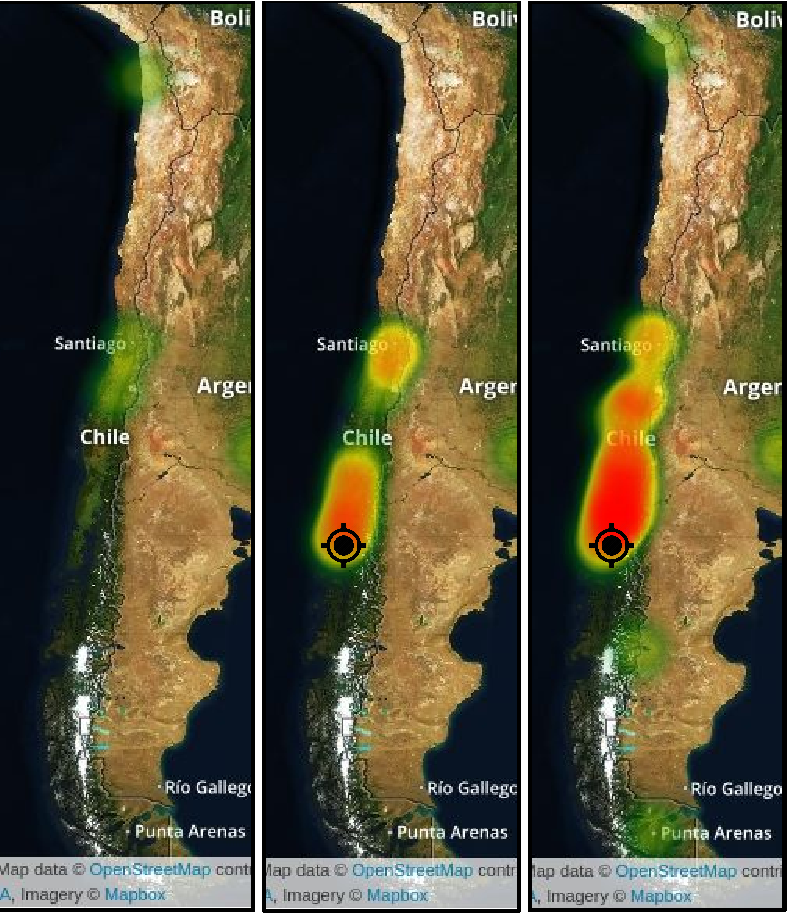
\includegraphics[trim={0 0 0 0}, clip, width=0.5\textwidth]{imagenes/heatmap.pdf}
	  \caption{Mapa de calor durante los primeros minutos posterior al inicio del sismo al norte de Melinka, Región de Aysén, Chile, el 25 de Diciembre del 2016.}
		\label{fig:heatmap-timelapse}
	\end{figure}	
	
	Durante el primer minuto posterior a la publicación del primer \textit{tweet} se publicaron 36 otros mensajes (sin contar \textit{retweets}). Además, luego de los primeros reportes, que generalmente son cortos y sin mucho detalle, se comienzan a compartir otros mensajes con información respecto a la intensidad del mismo. Mensajes cómo los presentados a continuación, ayudan a quien los lee, a entender que el sismo se percibió con una alta intensidad. 
	

\textit{``Hace mucho no sentía un temblor así'' $@$Estrella\_WTF, 14:26:00, 25/12/16}

\textit{``URGENTE Fuerte sismo se siente en \#Coyhaique'' $@$Radio45Sur, 14:26:00 25/12/16}

\textit{``Sendo temblor wn'' $@$goodzquad, 14:26:00 25/12/16}

\textit{``Fuerte temblor en el sur. Aquí en Purranque se sintió con tuti!!'' $@$Cristianc78, 14:26:00 25/12/16}

	\begin{figure}[!h]
	  \centering
	  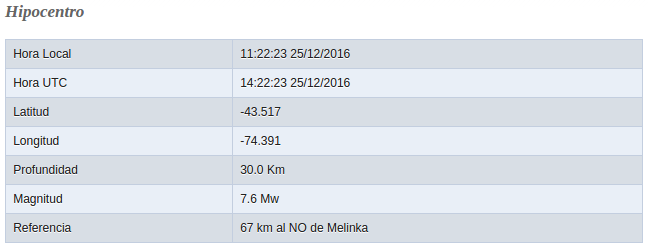
\includegraphics[trim={0 0 0 0}, clip, width=0.7\textwidth]{imagenes/img-25Dic-Hipocentro.png}
	  \caption{Vista de la aplicación Web disponible públicamente}
		\label{fig:25dic-hipocentro}
	\end{figure}
	
	La geolocalización de \textit{tweets} permitió presentar visualmente la zona en la cual las personas eran capaces de percibir movimiento. Las figuras \ref{fig:heatmap-timelapse} presentan la variación de las visualizaciones geográficas durante los primeros 5 minutos. En base a estas imágenes, es fácil inferir que el sismo fue percibido cerca de las regiones de Aysén y Los Ríos, ya que es en esa zona donde aparecen las primeras publicaciones. También se observa que al transcurrir los minutos, las personas comienzan a publicar mensajes desde zonas más alejadas. Esto se debe a dos razones principales, que la onda del sismo se percibe en diferentes instantes de tiempo dependiendo de la distancia focal y porque la noticia se difunde rápidamente a través de la red social. En este caso en particular, se observan mensajes en Santiago, sin embargo, el sismo fue percibido con muy baja intensidad en la Región Metropolitana, por lo que se infiere que esos \textit{tweets} corresponden a mensajes de difusión y que las personas no se encuentran necesariamente en el radio de percepción del sismo.
		
	La información oficial dispuesta por el Centro Sismológico Nacional (CSN) detalla que el epicentro del sismo se encuentra a 67 Km al Noroeste de Melinka, Región de Aysén, a 30 Km de profundidad y que la magnitud del sismo fue de 7,6 Mw. Lo que confirma lo inferido en base a las visualizaciones presentadas en la aplicación. La tabla de la figura \ref{fig:25dic-hipocentro} muestra otros detalles presentados por las fuentes oficiales. 
	Mientras este reporte fue publicado a pocos segundos del suceso, el informe preparado por la Oficina de Análisis en relación a la {\em intensidad}, es decir, el efecto que el sismo tuvo en la superficie y el alcance que tuvo en los pueblos de la zona, fue publicado a las 12:26 hrs. (4 minutos luego de ocurrido el suceso).
	Por lo tanto, previo a la entrega de este informe oficial, la aplicación ayudó a estimar de forma preliminar la gravedad de la situación. 
	
	
Cabe destacar que aunque el hipocentro de este sismo se ubicaba al norte de Melinka y en la zona sur de la isla de Chiloé, la mayoría de los \textit{tweets} fueron publicados por personas ubicadas al norte del hipocentro, cerca de la zona norte de la isla de Chiloé y también en Puerto Montt. Esto se puede explicar debido a la menor población de esas ciudades, acompañado de la heterogeneidad del uso de Twitter y del acceso a internet que existe a lo largo de las diferentes regiones de Chile.
	

	\section{Caso II: Sismos en otros países}
	
	El sistema propuesto está pensado para detectar sismos en diferentes idiomas y/o países. A continuación se presentan algunos casos de sismos ocurridos en otros países.  
	
	\subsection{Sismo en México}
	
\begin{figure}[!h]
	  \centering
	  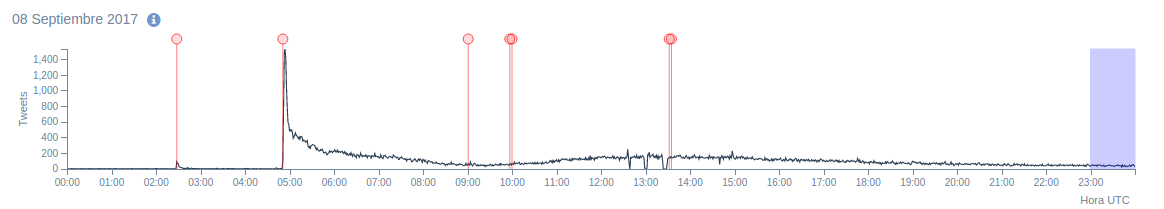
\includegraphics[width=\textwidth]{imagenes/img-sismo-mexico.png}
	  \caption{Frecuencia de mensajes relacionados con sismos durante el 8 de Septiembre del 2017.}
		\label{fig:timeline-mexico}
\end{figure}	
		
El terremoto de Chiapas de 2017 ocurrido 04:49:18, del jueves 8 de Septiembre (hora UTC). Tuvo una magnitud de 8,1 Mww, según el Servicio Geológico de los Estados Unidos (USGS)). El epicentro se ubicó en el Golfo de Tehuantepec, 137 km al suroeste de Pijijiapan (Chiapas), y a 69,7 km de profundidad. El sismo se percibió en el centro y sureste de México, así como en Guatemala, El Salvador, Honduras y Bélice.

	El sistema fue capaz de detectar este sismo sin problemas y debido a su gran intensidad se observó mucho ruido en la aplicación Web durante las horas posteriores al evento. La figura \ref{fig:timeline-mexico} muestra la frecuencia de mensajes el día 8 de Diciembre (Hora UTC). En las figuras \ref{fig:worldmap-mexico} y \ref{fig:worldmap-zoom-mexico} se puede observar cómo el sistema es capaz de informar acerca del lugar del evento y de otros lugares en los que este fue percibido. 
	
		\begin{figure}[!h]
\minipage{0.46\textwidth}
 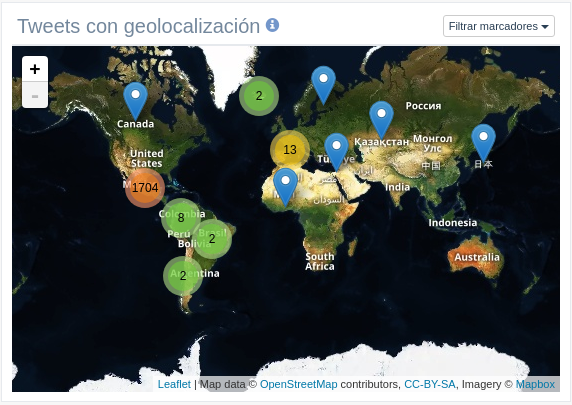
\includegraphics[width=\textwidth]{imagenes/img-worldmap-mexico.png}
	  \caption{Mapa del mundo con marcadores para los \textit{tweets} geolocalizados publicados durante los primeros minutos posteriores al inicio del sismo ocurrido en Chiapas, México en Semptiembre del 2017.}
		\label{fig:worldmap-mexico}
\endminipage\hfill
\minipage{0.46\textwidth}
 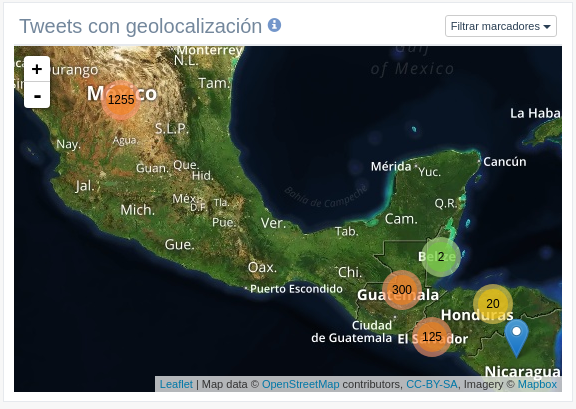
\includegraphics[trim={0 0 0 0}, clip, width=\textwidth]{imagenes/img-worldmap-zoom-mexico.png}
	  \caption{Mapa con marcadores para los \textit{tweets} geolocalizados, con zoom en la zona afectada,  publicados durante los primeros minutos posteriores al inicio del sismo ocurrido en Chiapas, México en Semptiembre del 2017.}
		\label{fig:worldmap-zoom-mexico}
\endminipage\hfill
\end{figure}
	
	\subsection{Sismo en Italia}
	
	\begin{figure}[!h]
	  \centering
	  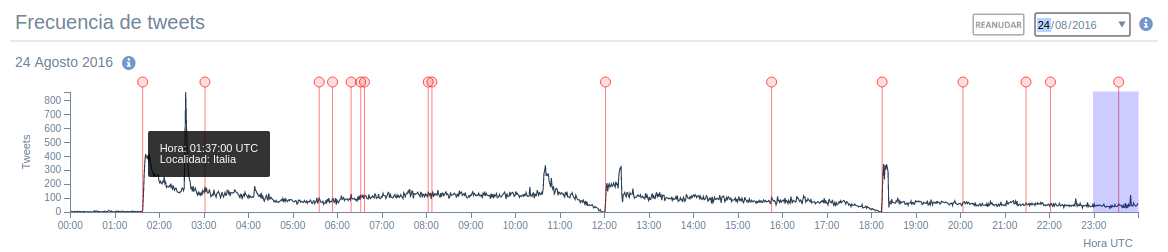
\includegraphics[width=\textwidth]{imagenes/sismoitaliafreq.png}
	  \caption{Frecuencia de mensajes relacionados con sismos durante el 24 de Agosto del 2016.}
		\label{fig:timeline-italia} 
	\end{figure}
	
	El día 24 de Agosto del 2016 a las 01:36 UTC, ocurrió un sismo muy fuerte en Italia central. Dada la magnitud del evento, el cual se registró con una magnitud de 6.2 Mw, el sistema fue capaz de detectarlo en menos de un minuto luego de la publicación del primer \textit{tweet}. Al observar la frecuencia de \textit{tweets} para ese día (figura \ref{fig:timeline-italia}), se observa una curva muy ruidosa y algunos picos que coinciden con los momentos importantes a lo largo del desarrollo de las actividades de recuperación. Muchos de los marcadores rojos dibujados a lo largo del día muestran momentos en los cuales hubo variaciones en la frecuencia, pero no necesariamente debido a un sismo, si no más bien, a puntos en donde se anunciaron los daños producidos. También hay depresiones abruptas en la frecuencia que se deben a las restricciones impuestas por Twitter debido al gran flujo de mensajes que se estaban recolectando. 
	
	El primer mensaje que hace alusión al sismo fue publicado a las 01:37 UTC y durante los primeros 5 minutos posteriores se publicaron aproximadamente 2000 \textit{tweets} que mencionan palabras clave relacionadas con sismos (sin contar \textit{retweets}). De estos, aproximadamente 885 mensajes fueron geolocalizados y en la figura \ref{fig:sismoitalia} se puede ver claramente que la mayoría de ellos fueron publicados desde Italia.
	
	\begin{figure}[!h]
	  \centering
	  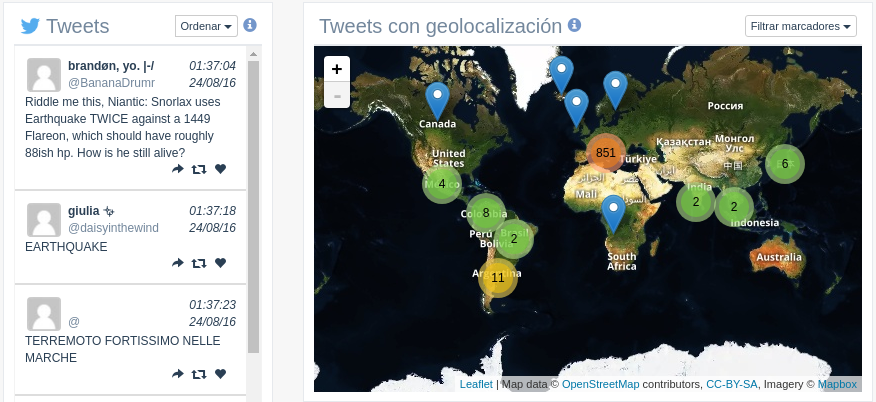
\includegraphics[width=\textwidth]{imagenes/sismoitalia.png}
	  \caption{Distribución de los mensajes publicados durante los primeros 10 minutos posterior al inicio del sismo en Italia central el 24 de Agosto del 2016.}
		\label{fig:sismoitalia}
	\end{figure}	
	
	La gravedad de la situación posterior al evento se reflejó en la red social, ya que durante el día, se continuaron publicando aproximadamente 100 mensajes por minuto haciendo referencia a sismos. Este comportamiento continuó hasta el día 25 de Agosto. Además, durante este periodo, los mensajes eran publicados desde diferentes países del mundo, demostrando ser un evento de interés internacional.
	
	
	\subsection{Otros Ejemplos}
	
	
	La figura \ref{fig:timeline-26Oct} muestra la frecuencia de \textit{tweets} del 26 de Octubre del 2016. Durante este día ocurrieron varios sismos en diferentes países y la herramienta fue capaz de detectarlos correctamente. 
	
	\begin{figure}[!h]
	  \centering
	  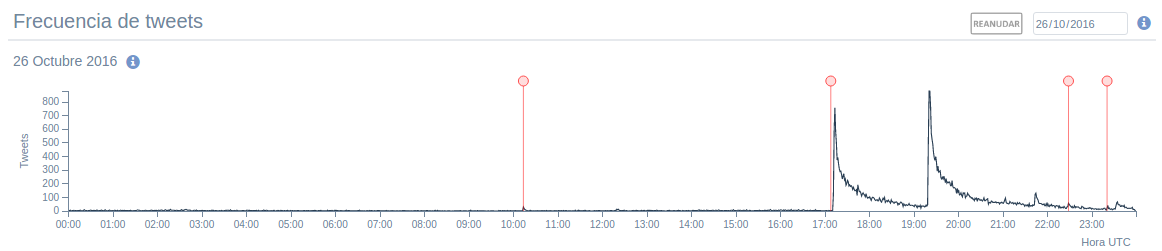
\includegraphics[width=\textwidth]{imagenes/26Octubrefreq.png}
	  \caption{Frecuencia de mensajes relacionados con sismos durante el 26 de Octubre del 2016.}
		\label{fig:timeline-26Oct}
	\end{figure}
	
	La primera detección que se visualiza en la aplicación Web ocurrió a las 10:13 UTC. Al seleccionar el rango de los 5 min posteriores se puede observar las visualización que se presenta en la imagen \ref{fig:sismojapon}. En la imagen se puede identificar que el evento ocurrió en Japón. La baja frecuencia asociada al evento se debe a que la aplicación Web muestra los datos filtrados por idiomas y este filtro no incluye el japonés, por lo que los \textit{tweets} visualizados corresponden únicamente a los escritos en inglés. 
	
	\begin{figure}[!h]
	  \centering
	  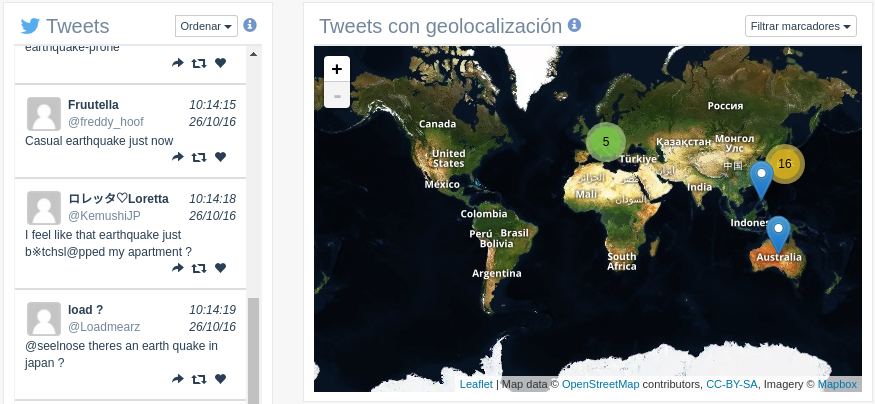
\includegraphics[width=\textwidth]{imagenes/sismoJapon.png}
	  \caption{Visualización de los mensajes publicados durante los primeros 5 minutos posterior al inicio de un sismo en Japón el 26 de Octubre del 2016.}
		\label{fig:sismojapon}
	\end{figure}
	
	
	La segunda detección ocurrida a las 17:07 UTC corresponde a un sismo en Italia y las ráfagas de \textit{tweets} que se observan a las 19:19 UTC y a las 21:43 UTC corresponden a otros sismos en Italia. En la visualización el segundo y tercer sismo no tienen marcadores. Este caso en el que sismos posteriores ocurridos en el mismo país no se marcan, se debe a que la velocidad de publicación de \textit{tweets} no alcanzó a decrecer lo suficiente antes de ocurrido el siguiente sismo y tampoco se mencionan nuevos países, por lo tanto se consideran como un mismo evento. 

	
	Al seleccionar los periodos de 5 min posterior a cada sismo se observa claramente el lugar donde ocurre el sismo y los tres eventos están ubicados en la península de Italia.
	
	\begin{figure}[ht]
	\centering
	\subfloat[Sismo detectado a las 17:07 UTC del 26 de Octubre del 2016.]{
		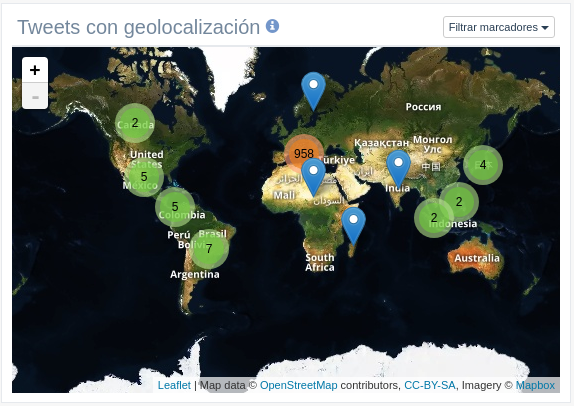
\includegraphics[width=140pt]{imagenes/sismoitalia-1.png}
		\label{fig:sismoitalia1}
	}
	\hfill
	\subfloat[Sismo detectado a las 19:19 UTC del 26 de Octubre del 2016.]{
  		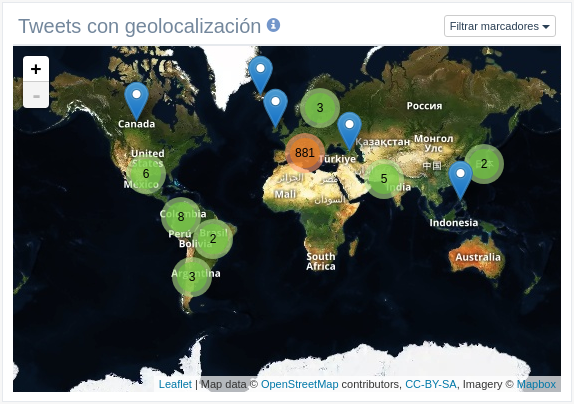
\includegraphics[width=140pt]{imagenes/sismoitalia-2.png}
  		\label{fig:sismoitalia2}
  	}
  	\hfill
	\subfloat[Sismo detectado a las 21;43 UTC del 26 de Octubre del 2016.]{
  		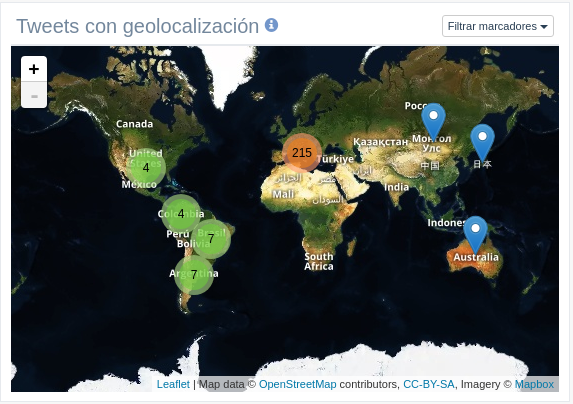
\includegraphics[width=140pt]{imagenes/sismoitalia-3.png}
  		\label{fig:sismoitalia3}
  	}
  	\caption{Distribución geográfica de los \textit{tweets} publicados en los 10 minutos posteriores a cada uno de los sismos detectados desde las 17:07 y las 21:43 del 26 de Octubre del 2016.}
  	\label{fig:sismoitaliamult}
  	\end{figure}
	
	La tercera detección ocurrida a las 22:28 UTC, se observa con una frecuencia muy baja. Al seleccionar el rango posterior a la detección se puede observar la distribución de los mensajes en el mapa y tal como se muestra en la imagen \ref{fig:sismocostarica-world}, aun existe una concentración importante de mensajes en Italia, pero también hay un grupo en la zona de América Central. Al acercar la imagen al sector de América Central \ref{fig:sismocostarica-zoom} se ve claramente que un sismo ha ocurrido en Costa Rica. 
	
	
	\begin{figure}[ht]
	\centering
	\subfloat[Mapa del mundo]{
		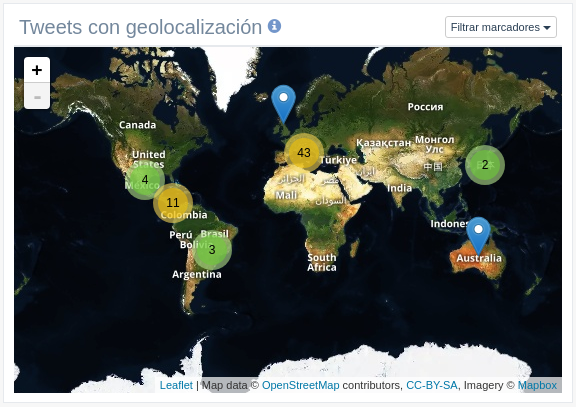
\includegraphics[width=220pt]{imagenes/sismocostarica1.png}
		\label{fig:sismocostarica-world}
	}
	\hfill
	\subfloat[Ampliación América Central]{
  		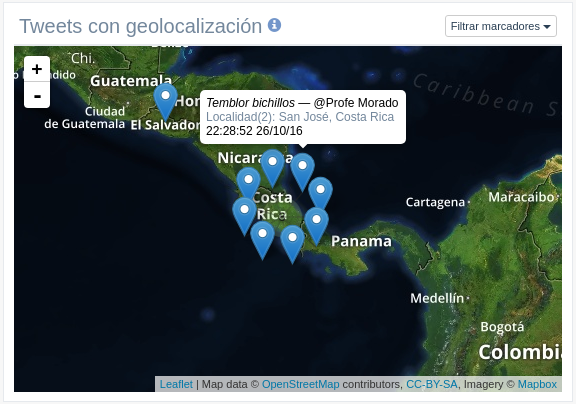
\includegraphics[width=220pt]{imagenes/sismocostarica.png}
  		\label{fig:sismocostarica-zoom}
  	}
  	\caption{Distribución de los \textit{tweets} publicados entre las 22:28 y las 22:38 UTC el 26 de Octubre del 2016.}
  	\label{fig:sismocostarica}
  	\end{figure}
	
	Finalmente, la última detección del día a las 23:20 UTC, tal como muestra la imagen \ref{fig:sismomexicoleve}, corresponde a un sismo en México. 
	
	\begin{figure}[!h]
	  \centering
	  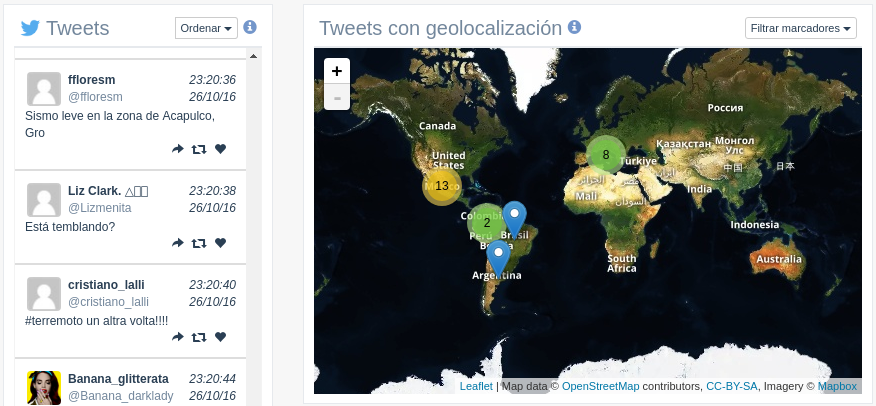
\includegraphics[width=\textwidth]{imagenes/sismomexicoleve.png}
	  \caption{Visualización de los mensajes publicados durante los primeros 5 minutos posterior al inicio de un sismo en México el 26 de Octubre del 2016.}
		\label{fig:sismomexicoleve}
	\end{figure}
	
	 
	\subsection{Observaciones}	 
	
	Para estos casos es interesante observar, que dependiendo del país en el que ocurre el sismo y de la intensidad de este, el ruido y el periodo de tiempo en el cual los usuarios de la red social continúan hablando del suceso puede variar desde un par de horas hasta incluso varios días.
	
	\section{Caso III: Falsos Positivos}
	\label{sec:casosfalsos}
	
	\begin{figure}[h]
	  \centering
	  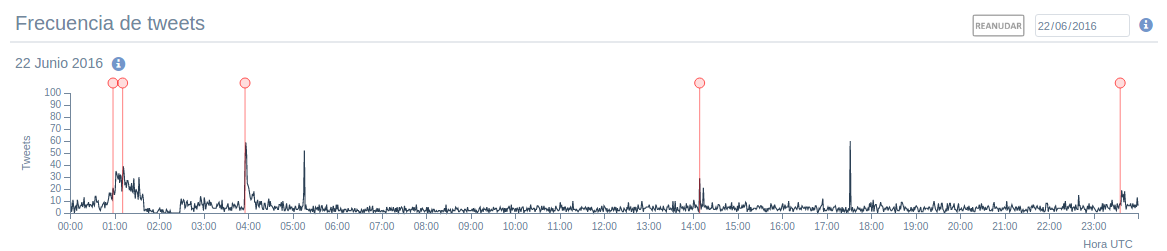
\includegraphics[trim={0 0 0 0}, clip, width=\textwidth]{imagenes/22junio2016-freq.png}
	  \caption{Frecuencia de mensajes relacionados con sismos durante el día 22 de Junio del 2016.}
		\label{fig:timeline-22junio}
	\end{figure}	
	
	Durante el periodo en el que el sistema ha estado disponible se han identificado algunos casos de detecciones falsas. El caso aquí presentado corresponde a un simulacro de sismo ocurrido en Filipinas el año 2016. Este simulacro, al ser de carácter masivo, ocasionó que muchas personas compartieran en la red social comentarios respectivos a su realización más o menos al mismo tiempo, de forma similar a como ocurre durante un evento sísmico real. En la imagen \ref{fig:timeline-22junio}, las dos primeras detecciones de ese día corresponden a falsos positivos. En este caso, la distribución de la frecuencia de \textit{tweets} es diferente a la que se observa durante un sismo real. Al seleccionar el rango de tiempo, se puede ver lo que se muestra en la figura \ref{fig:earthquakedrill}. En esta visualización se observa que los mensajes se geolocalizan en Filipinas por lo que se podría pensar que corresponde a un evento real, sin embargo, al revisar en detalle lo que dicen los mensajes, se menciona ``\textit{earthquake drill}'' lo que en español significa ``simulacro de terremoto''. 
	
	\begin{figure}[h]
	  \centering
	  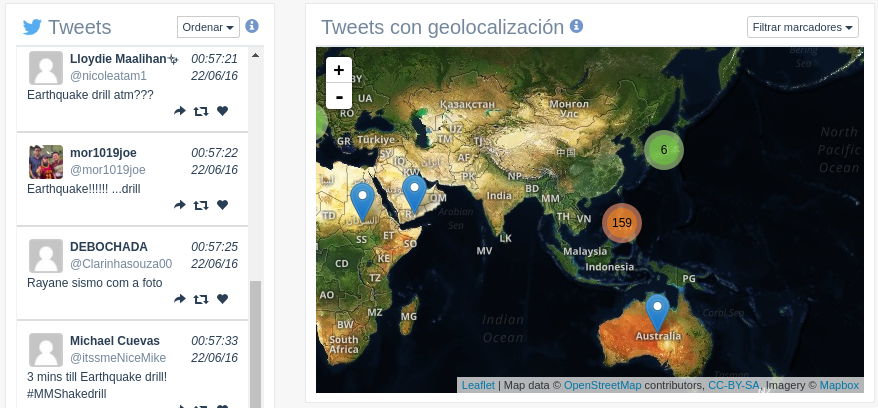
\includegraphics[width=\textwidth]{imagenes/earthquakedrill.png}
	  \caption{Visualización de los mensajes publicados entre las 00:45 y las 01:30 el 22 de Junio del 2016, durante un simulacro de sismo en Filipinas.}
		\label{fig:earthquakedrill}
	\end{figure}	
	
	A pesar de que se identificaron casos de ese tipo, al presentar características muy similares a las de un sismo real, no se tomaron medidas para filtrarlos. Sin embargo, gracias a la disposición de los elementos en la aplicación Web, se puede identificar fácilmente, mediante la lectura de algunos de los mensajes publicados, que no se trata de un sismo real, si no más bien de un simulacro masivo. 
	
	
\section{Conclusión}
\label{sec:conclusion}

\jm{agregar conclusión}
	